% DIAPOSITIVA 21 (renumerada): Escalera de modelos
\begin{frame}{Escalera de modelos (P3)}
  {\small\textbf{Desempeño fuera de muestra (LOCO-CV, 31 contiendas)}}
  \vspace{0.15em}
  \begin{center}
  {\setlength{\tabcolsep}{4pt}
  \small
  \rowcolors{2}{tableBand}{white}
  \begin{tabular}{L{4.5cm} C{2.0cm} C{1.8cm} C{1.8cm}}
    \toprule
    \rowcolor{barBlue}
    {\color{white}\textbf{Modelo}} &
    {\color{white}\textbf{MAE}} &
    {\color{white}$R^2_{\text{oos}}$} &
    {\color{white}\textbf{Top-1}} \\
    \midrule
    Baseline proporcionalidad & 12,61 pp & 0,185 & 71,0\% \\
    Núcleo digital ($f_\ell$ solo) & 11,52 pp & 0,460 & 71,0\% \\
    \textbf{ElasticNet 2 variables} & \textbf{9,56 pp} & \textbf{0,518} & \textbf{64,5\%} \\
    Gradient boosting (ctrl) & 9,91 pp & 0,515 & 67,7\% \\
    \bottomrule
  \end{tabular}}
  \end{center}
  \vspace{0.2em}
  {\footnotesize Top-1 al 64,5\%: cuota de magnitud y acierto de orden son objetivos distintos.
  Top-1 es métrica derivada de la regresión, no un clasificador entrenado \corr{[1.20]}.}

  \vspace{0.3em}
  \begin{center}
    
\includegraphics[width=0.52\textwidth]{img/col_mae_escalera.png}
  \end{center}
\end{frame}

% DIAPOSITIVA 22 (renumerada): Curva de aprendizaje
\begin{frame}{Curva de aprendizaje (P4)}
  \begin{columns}[T]
    \begin{column}{0.40\textwidth}
      \begin{center}
      \small
      \rowcolors{2}{tableBand}{white}
      \begin{tabular}{C{2.2cm} C{1.8cm} C{1.4cm}}
        \toprule
        \rowcolor{barBlue}
        {\color{white}\textbf{Ciudades}} &
        {\color{white}\textbf{MAE medio}} &
        {\color{white}\textbf{DE}} \\
        \midrule
        5  & 12,82 pp & 1,37 \\
        10 & 12,53 pp & 1,07 \\
        15 & 12,45 pp & 0,94 \\
        20 & 12,22 pp & 0,84 \\
        30 & 12,05 pp & 0,00 \\
        \bottomrule
      \end{tabular}
      \end{center}
      \vspace{0.4em}
      \begin{exampleblock}{\textbf{P4}: Respondida}
        Con 10 ciudades se alcanza el 95\% del rendimiento final.
        El piso de error es \textbf{estructural} (ruido de señal),
        no insuficiencia de datos.
      \end{exampleblock}
    \end{column}
    \begin{column}{0.56\textwidth}
      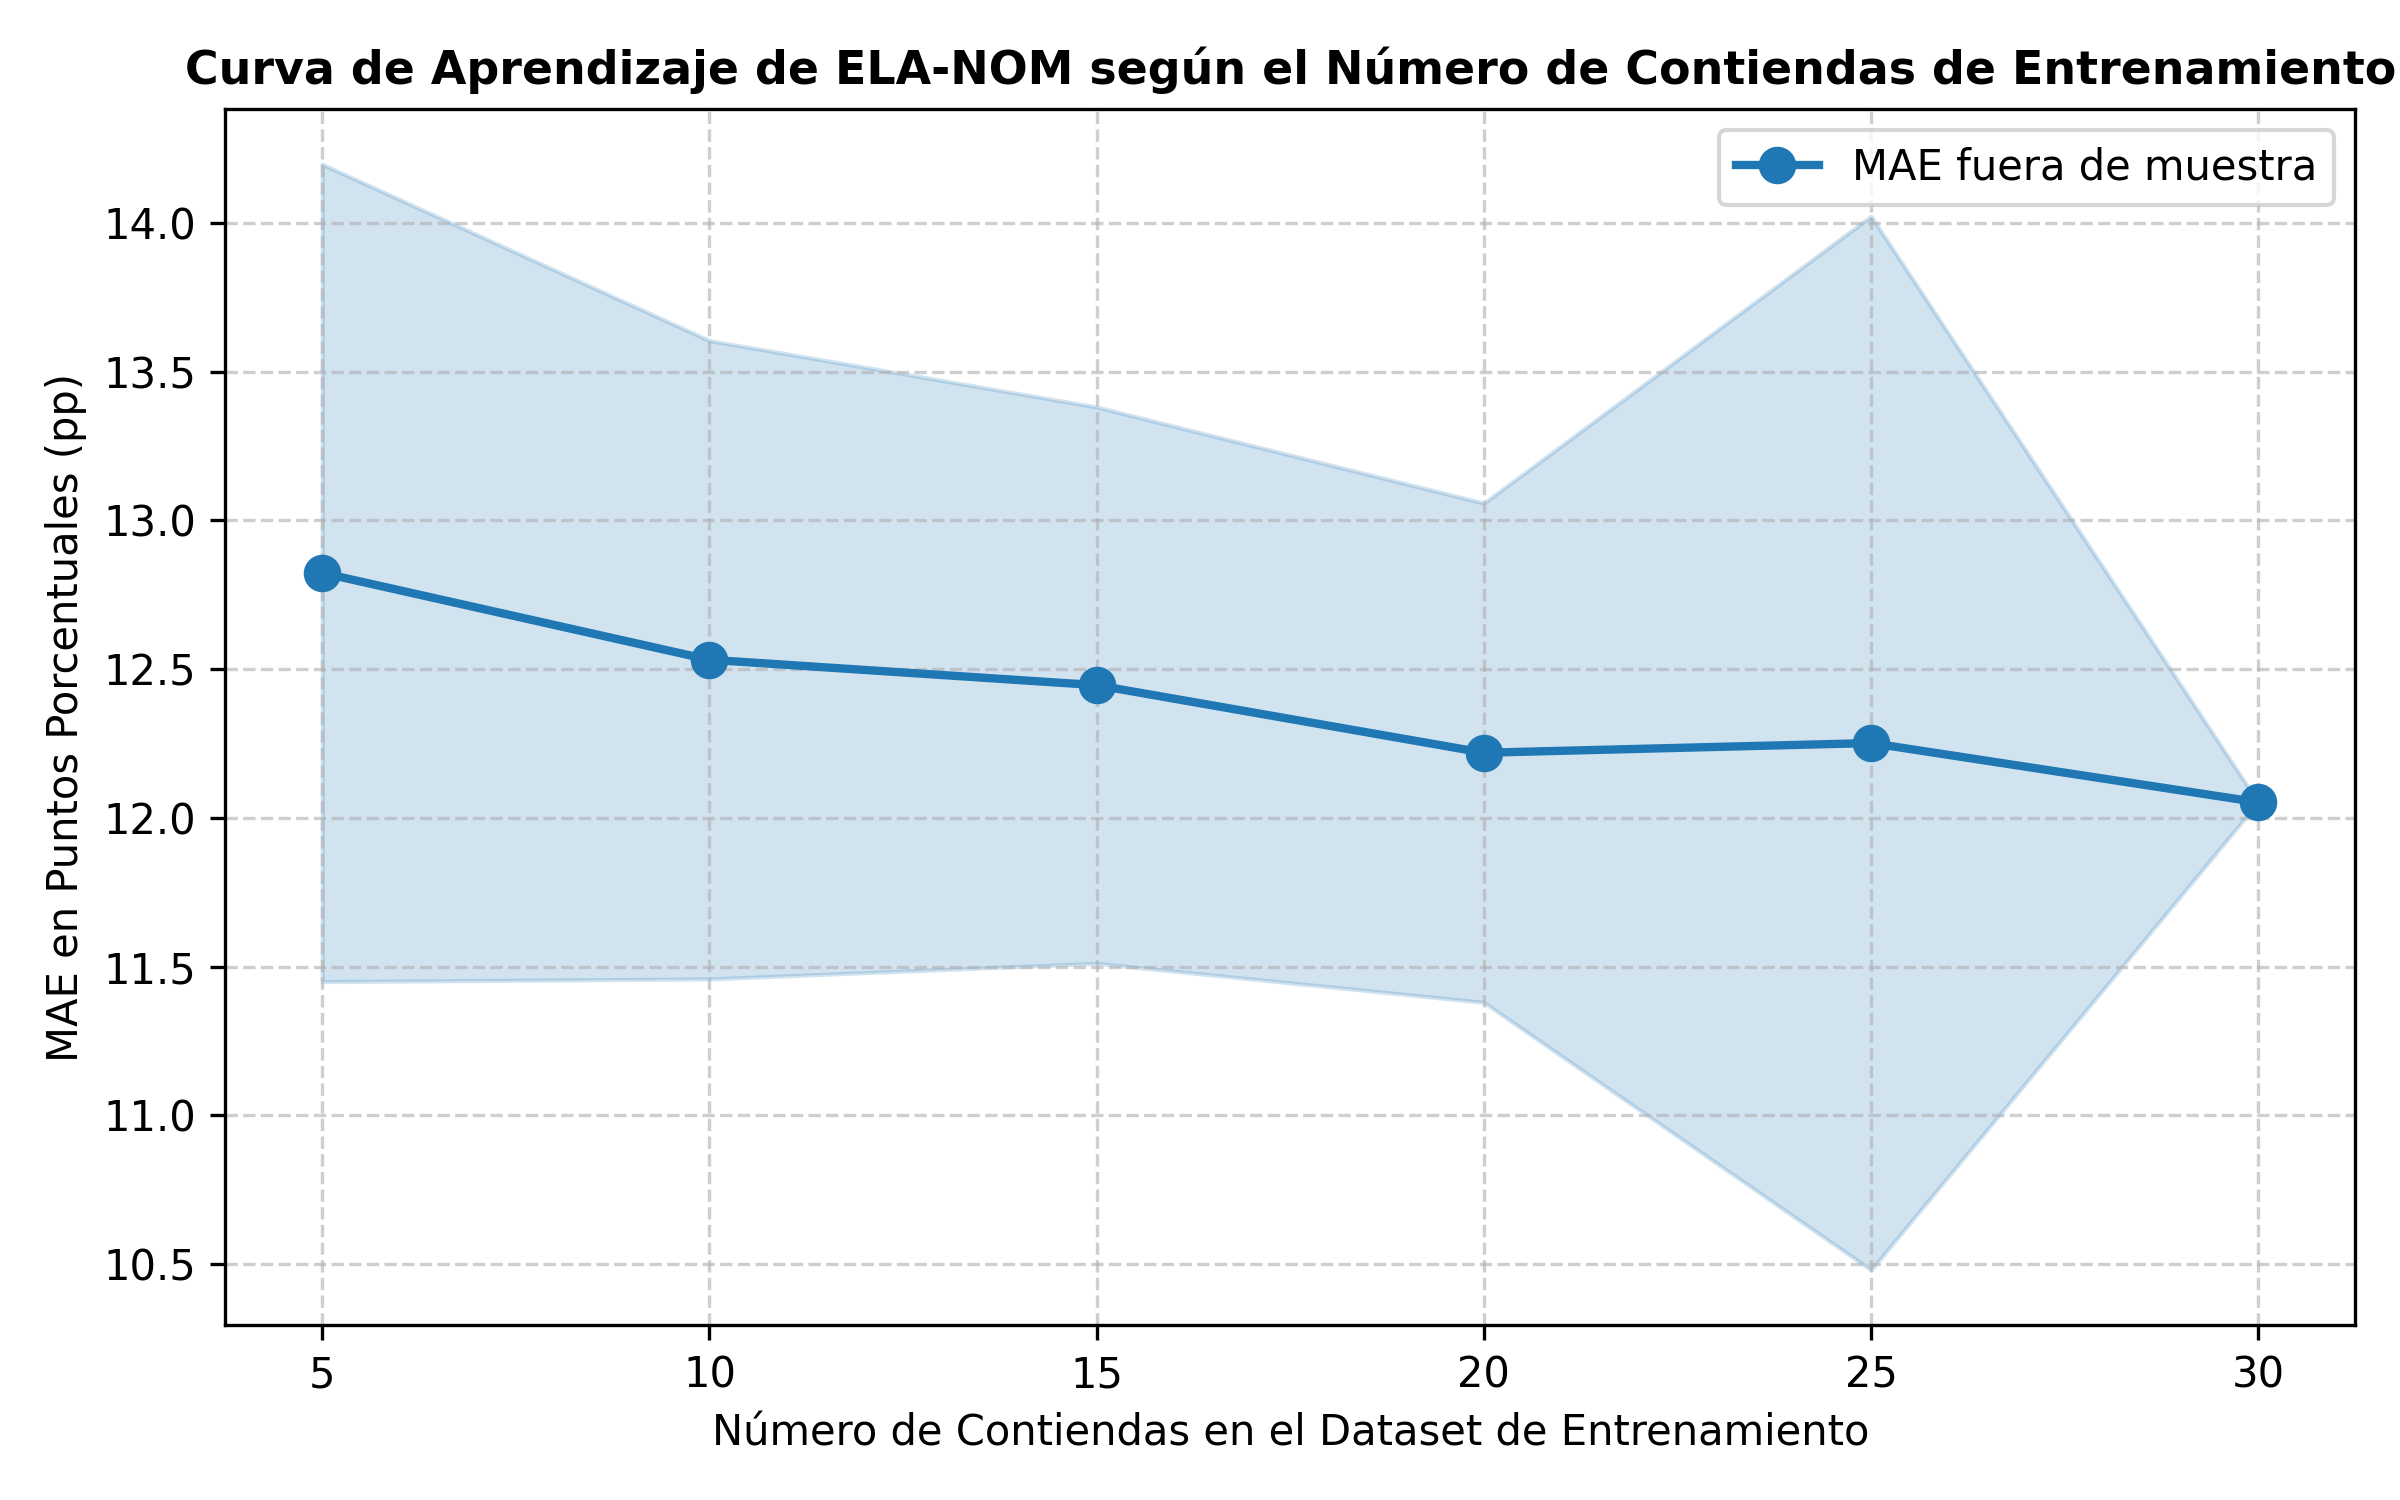
\includegraphics[width=\textwidth]{img/col_learning_curve.png}
    \end{column}
  \end{columns}
\end{frame}

% DIAPOSITIVA 23 (renumerada): Validación 2026 -- datos
\begin{frame}{Validación prospectiva: 2.ª vuelta presidencial 2026}
  \begin{columns}[T]
    \begin{column}{0.52\textwidth}
      \textbf{Cepeda Castro vs.\ De la Espriella}, 21 jun.\ 2026

      \vspace{0.2em}
      \begin{center}\small
      \rowcolors{2}{tableBand}{white}
      \begin{tabular}{L{2.6cm} R{2.2cm} C{1.6cm}}
        \toprule
        \rowcolor{barBlue}
        {\color{white}\textbf{Candidato}} &
        {\color{white}\textbf{Total \textit{likes}}} &
        {\color{white}\textbf{Dom.}} \\
        \midrule
        Cepeda Castro   & 17.087.679 & \num{77,6\%} \\
        De la Espriella &  4.926.361 & \num{22,4\%} \\
        \bottomrule
      \end{tabular}
      \end{center}
      \vspace{0.2em}
      \textbf{Corrección metodológica:}\\
      {\small Modelo entrenado: base aprox.\ 26\% (3,84 candidatos prom.)\\
      2.ª vuelta: base = 50\%; se elimina intercepto:}
      \[
        \hat{p}_c^{(2)} = 0{,}50 + \hat\beta_1 \cdot f_\ell(c)
      \]
      \textbf{Pronósticos:}
      $\hat{p}_{\text{Cepeda}} = \num{60{,}5\%}$,
      $\hat{p}_{\text{Espriella}} = \num{39{,}5\%}$

      \vspace{0.2em}
      {\small \textbf{Trazabilidad} \corr{[Corr.\ 1.15]}: 14 días previos, FB+TW+TikTok,
      444 publicaciones, ElasticNet 2v.\ (random\_state=42)}
    \end{column}
    \begin{column}{0.44\textwidth}
      
\includegraphics[width=\textwidth]{img/col_dominancia_2026.png}
      {\footnotesize\color{subtleGray} Dominancia de \textit{likes}, 444 publicaciones}

      \vspace{0.4em}
      \begin{exampleblock}{\textbf{PM4}: Respondida}
        \small El modelo es \textbf{transferible} a un formato electoral diferente:
        elección presidencial bipolar vs.\ alcaldías multicandidate.
      \end{exampleblock}
    \end{column}
  \end{columns}
\end{frame}

% DIAPOSITIVA 24 (renumerada): Resultado 2026 + corrección MAE
\begin{frame}{Resultado real: contextualización del error \corr{[Corr.\ 1.17/2.4]}}
  \begin{columns}[T]
    \begin{column}{0.52\textwidth}
      \textbf{Resultado real (21 jun.\ 2026):}
      \[
        \text{De la Espriella: } 50{,}48\%
        \quad
        \text{Cepeda: } 49{,}52\%
      \]
      Margen real: \alrt{\textbf{0,96 pp}}, empate técnico.

      \vspace{0.2em}
      \[
        \text{MAE}_{2026} = |60{,}5\% - 49{,}52\%| = \num{10{,}98\,\text{pp}}
      \]
      Supera el MAE medio de entrenamiento en $+1{,}42$ pp.

      \vspace{0.2em}
      \begin{alertblock}{Corrección conceptual: $\pm$MAE no es intervalo}
        \small El MAE mide exactitud promedio, no dispersión.
        ``$\hat{p} \pm \text{MAE}$'' \textbf{no tiene cobertura estadística declarada}.
        Un intervalo formal requiere percentiles de los residuos de LOCO-CV
        o supuestos distribucionales explícitos.
      \end{alertblock}
    \end{column}
    \begin{column}{0.44\textwidth}
      \textbf{Límite estructural:}
      \begin{itemize}\small
        \item Cepeda acumuló 3,5 veces más \textit{likes}; señal real y robusta
        \item Ningún modelo de engagement resuelve contiendas menores a 1 pp
        \item Las encuestadoras colombianas tampoco lo lograron
        \item Factores no capturados: movilización territorial, giros de última semana
      \end{itemize}
      \vspace{0.3em}
      \begin{block}{Uso práctico adecuado del modelo}
        \small ELA-NOM es informativo para ordenar tendencias y detectar
        ventajas mayores a 20 pp. \textbf{No} está diseñado para predecir
        empates técnicos.
      \end{block}
      \vspace{0.2em}
      \begin{exampleblock}{\textbf{PM4}: Delimitado}
        \small El fallo es una condición de borde (margen menor a 1 pp),
        no una falsación del modelo.
      \end{exampleblock}
    \end{column}
  \end{columns}
\end{frame}
